\subsection{Radiation System Design}
\label{sec:Radiation-Design}

\subsubsection{Radiation Monitoring}
The radiation monitoring system consists of the two Timepix devices.
Each device was placed in separate structures in order to compare the recorded data between devices and to data from previous flights, allowing us to determine effectiveness of the constructed ISS container.
The FITPix was placed within a container exactly resembling the contained used for the previous two SORA experiments and acted as the control during the 2019 mission.
The MiniPIX was placed inside the mock-up ISS module for two primary reasons.
The first being that it would allow a direct comparison between the 2019 data and the data from the previous two SORA missions, since the previous missions used the exact same MiniPIX in the exact same configuration.
The second reason was to protect the FITPix.
The FITPix used in the SORA 3 mission was a borrowed device, and placing this borrowed device in the new, untested ISS module was deemed inappropriate.

The work of the first two SORA experiments \cite{SORA1} \cite{SORA2} established a strong foundation for the radiation dosimetry portion of the experiment.
The software used to control the devices was an extension of the previous year's software with the key difference being that this year's software could accommodate two Timepix devices rather than one. 
The flight computer had a main thread in which controlled and monitored the entire payload, and new, separate threads would be created to gather the Timepix data so that the sensors and the uplink/downlink connection could be maintained while gathering Timepix data.
Once the Timepix data was collected, it would be analyzed in real-time and the particle counts and dose would be sent as part of the downlinked data packet. 

% Section for the FITPix configuration (including figure(s))
The primary structure of the FITPix container was 3D printed using ABS plastic, which is consistent with previous missions.
The choice to use 3D printed material is backed by the need to minimize parts needed to construct the container.
By minimizing the parts, specifically metal parts, the interactions between the primary particles and the material of the structure are minimized.
Ideally, the device would be directly exposed to the atmosphere, but the container is needed to protect the device during landing. 
There was no concern of the plastic structure becoming compromised since this material has been tested during previous flights and a large heatsink is used to keep the device cool.
Shown in Figure \ref{fig:fitpix-container}, two aluminum blocks are used as heatsinks.
The device was secured to the smaller block with thermal paste, and the smaller block was secured to the larger piece with thermal paste. 

\begin{figure}[h!]
	\begin{center}
		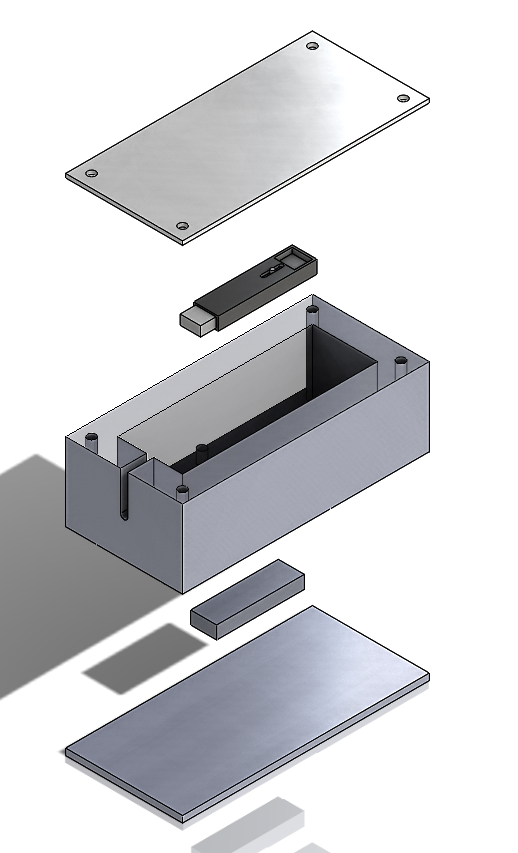
\includegraphics[width=0.5\textwidth]{figures/fitpix-case-exploded.png}
		\caption{Exploded view of the FITPix case assembly.}
		\label{fig:fitpix-container}
	\end{center}
\end{figure}

% Section for the MiniPIX configuration (including figure(s))
As previously mentioned, the MiniPIX was placed within the mock-up ISS module.
The module was constructed using the materials and material proportions given by Ref. \cite{NASA-ISS-Construction}.
The description of the module layers can be seen in Figure \ref{fig:iss-module}.
Aluminum 2219-T87 is aircraft grade material, is very expensive (on the order of several thousand dollars), and can only be ordered in bulk.
Due to monetary constraints, it was replaced with aluminum 6061-T6, but the dimensions were kept the same.
% Manufacturing the ISS module
%The ISS module was constructed layer by layer.
The inner-most (atmosphere-containing) aluminum structure was constructed by cutting sheets for each face of the box then welding the pieces together to form the box.
%This structure was then wrapped by the kevlar fabric.
%With the thickness of the fabric ordered, 
The front face of the box was left open to allow access to the inside of the structure.
In order to simulate the ISS environment as closely as possible, the module was to be pressurized at one atmosphere.
This was to be accomplished by sealing gaps in the structure with a vacuum epoxy once the entire system was assembled.
To measure pressure and temperature inside the module, a sensor was placed inside with wires fed through the layers and sealed with epoxy.

\begin{figure}[h!]
	\begin{center}
		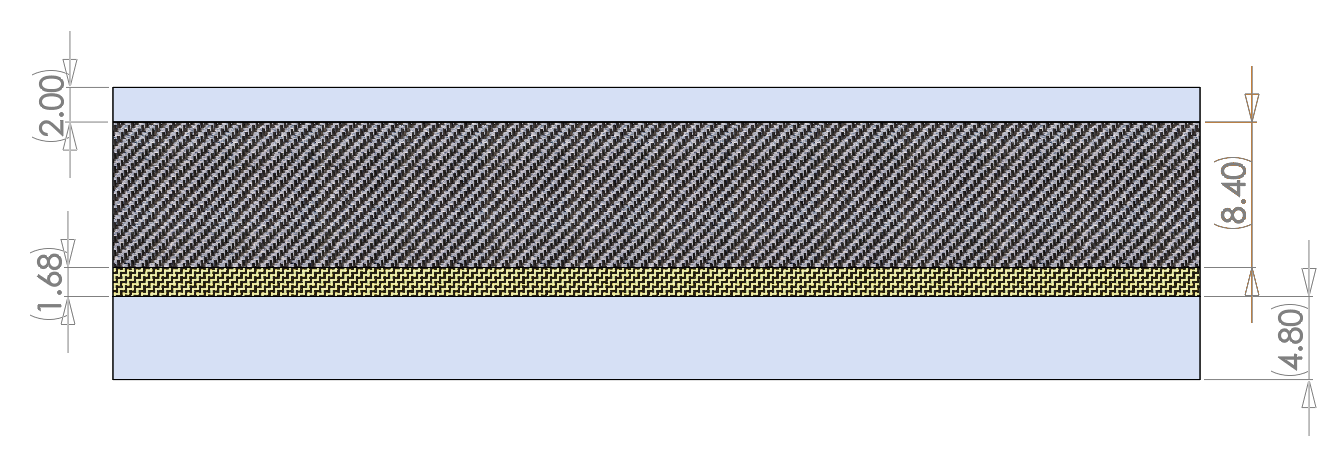
\includegraphics[width=\textwidth]{figures/iss-cross-section.png}
		\caption{Layers and thicknesses of the materials that will be used to construct the ISS module. From top to bottom: aluminum 6061-T6, six layers of Nextel AF62, six layers of Kevlar fabric, and aluminum 2219-T87. The atmosphere is contained by the 4.8 mm layer of aluminum. All dimensions are in mm.}
		\label{fig:iss-module}
	\end{center}
\end{figure}

\subsubsection{Organic Solar Cells}

The radiation group felt it would be most productive and insightful to be able to fabricate our own cells for launch, as opposed to outsourcing the work to another institution/graduate students or purchasing pre-made cells. With this decision came the reality of learning and understand the functionality behind each layer in the PV stack. The work done by the radiation group over the course of the SORA 3 mission can be divided into three main phases:
	
	\begin{enumerate}
		\item Materials research/Lab search
		\item Device fabrication/encapsulation
		\item Launch/post-launch analyses 
	\end{enumerate}
	
	We continued to recruit new members while our team started reviewing literature on the fabrication and operation of OPV. Solar cells stacks are categorized by the order in which layers are deposited, either a normal or inverted geometry. The so-called normal geometry consists of a transparent conductive oxide(TCO) for the high work function negative electrode, a hole transporting layer(HTL), active layer, electron transport layer(ETL), and low work function positive electrode (typically a metal). The HTL and ETL work to create an electric field across the active layer to draw out free charges, which are then collected at each electrode. The inverted geometry is characterized by a high work-function, negative top electrode and a hole blocking layer(EBL) atop the positive TCO electrode. Our group adopted the inverted geometry for greater stability of high work function metals.\\
	
\subsubsection{Acive Layer}
	
	The greatest consideration is given to the selection of the active layer. The active layer serves the purpose of converting photons (electromagnetic waves) in electrons (useful work). This happens as the small molecules or conjugated polymers absorb photons with energy greater than their band gap, defined as the difference between the highest occupied molecular level (HOMO) and the lowest unoccupied molecular level (LUMO); in essence the valence and conduction bands of any semiconductor. When photons are absorbed, electrons are excited from the HOMO to the LUMO band in what is known as the donor. Unlike crystalline semiconductors where charge separation occurs instantly, in organic photoactive materials the electrons remain bound to the left over positive charge, known as the hole, due to Coulombic attraction. This bound electron-hole pair is known as the exciton. The acceptor material will have a LUMO band which is lower in energy than the donor's, causing band bending at the interface and allowing the electron to be separated from the exciton state. Excitons and free charges both have low mobility and short lifetimes within organic materials, thus low diffusion lengths. This means that interfacial domains must be within the nanometer range in order to effectively separate the free charges. This problem has been addressed through the introduction of the bulk heterojunction (BHJ) active layer in which the acceptor and donor molecules are mixed into a single active solution prior to thin film fabrication, resulting in much greater interfacial surface area. And ideal organic active layer would maximize the interfacial surface area while optimizing layer and device thickness for light absorption, exciton diffusion, and charge collection.\\
	
	In our search we identified many candidate materials for the acceptor and donor molecules but ultimately decided it would be best to focus on the most widely researched BHJ pair of the semi-crystalline polymer Poly(3-hexylthiophene-2,5-diyl)(P3HT) as our donor and the fullerene derivative [6,6]-Phenyl C61 butyric acid methyl ester(PCBM) as our acceptor.\\
	
\subsubsection{Transport Layers}
	
	With the selection of the active layer and the knowledge of the inverted geometry stack, every other layer follows naturally. For the EBL we selected a sol-gel titania (TiO$_2$) based off of literature search and professional recommendations. Flourine doped tin oxide (FTO) was selected for the TCO opposed to indium doped tin oxide (ITO) due to the high temperatures required for annealing of sol-gel titania EBL. The purpose of annealing the titania solution after film application is to change from the amorphous to the anatase phase. The copolymer Poly(3,4-ethylenedioxythiophene)-poly(styrenesulfonate) (PEDOT:PSS)is most commonly used as a transport layer along with the P3HT:PCBM BHJs and was thus chosen as our ETL.
	
\subsubsection{Electrodes}
	
	Platinum was selected as our high work function electrode due to availability. The difference between the work functions of platinum and FTO creating the field which causes carrier drift once charges are seperated at the P3HT:PCBM interface. With these selections, our completed stack becomes \linebreak glass/FTO/TiO$_2$/P3HT:PCBM/PEDOT:PSS/Pt as shown in the figure below. \\
	
\subsubsection{Fabrication Ready Lab Search}
	
	One of the greater challenges at the beginning of our mission was acquiring access to a lab with the proper equipment to fabricate the devices ourselves. This search proved difficult due to a combination of a lack of experienced technicians to teach our group the fabrication techniques needed for OPV, a majority of labs only had a portion of the equipment needed in order to fabricate a complete device stack, and the limited budget available to our group for acquisition of materials and for equipment usage. Eventually we were lucky enough to receive permission from Dr. Oomman Varghese to use the equipment and materials within the Nanomaterials and Devices Laboratory where graduate student Lily Schafer and Maggie were both gracious enough to teach our group thin film fabrication techniques  and provide insight into the working principles behind OPV. With all materials and equipment secured, the radiation team proceeded into the fabrication phase. \\
